\documentclass{article}

% if you need to pass options to natbib, use, e.g.:
% \PassOptionsToPackage{numbers, compress}{natbib}
% before loading nips_2016
%
% to avoid loading the natbib package, add option nonatbib:
% \usepackage[nonatbib]{nips_2016}

\usepackage[final]{nips_2016}

% to compile a camera-ready version, add the [final] option, e.g.:
% \usepackage[final]{nips_2016}

\usepackage[utf8]{inputenc} % allow utf-8 input
\usepackage[T1]{fontenc}    % use 8-bit T1 fonts
\usepackage{hyperref}       % hyperlinks
\usepackage{url}            % simple URL typesetting
\usepackage{booktabs}       % professional-quality tables
\usepackage{amsfonts}       % blackboard math symbols
\usepackage{nicefrac}       % compact symbols for 1/2, etc.
\usepackage{microtype}      % microtypography
\usepackage{graphicx}

\title{Binary Classification of Imbalanced data from Bosch Production Line}

% The \author macro works with any number of authors. There are two
% commands used to separate the names and addresses of multiple
% authors: \And and \AND.
%
% Using \And between authors leaves it to LaTeX to determine where to
% break the lines. Using \AND forces a line break at that point. So,
% if LaTeX puts 3 of 4 authors names on the first line, and the last
% on the second line, try using \AND instead of \And before the third
% author name.

\author{
    P-1: \ Xi Yang \ Liang Dong \ Weijie Zhou \ Yeojin Kim
}

\begin{document}
% \nipsfinalcopy is no longer used

\maketitle

\section{Background}
\subsection{Gradient boosting tree}


Gradient boosting tree is achieving wide attention in Kaggle competitions. The basic idea of gradient boosting tree is to fit a base tree learner to pseudo-residuals.
\begin{center}
$r_{im} =-[\frac{\delta F(y_{i},F(x_{i}))}{\delta F(x_{i})} ]_{F(x)=F_{m-1}(x))}, i=1,...n$
\end{center}

Then computer $r_{m}$ by solving the following one-dimensional optimization problem:
\begin{center}
$\sum_{i=1}^{n}L(y_{i},F_{m-1}(x)+rh_{m}(x_{i}))$
\end{center}


And there are many versions of gradient boosting tree. In this paper, we will list five different versions of gradient boosting tree. 

Scikit Learn gradient boosting tree: implemented in python and integrated in scikit learn package, relatively slow 

SAS Viya: implemented in C and MPI, developed by SAS, supports python and lua API. It only support equal binning now.

xgboost(\url{https://github.com/dmlc/xgboost}): C language, open sourced and supply good support with python wrapper and R wrapper.

FastBDT(\url{https://github.com/thomaskeck/FastBDT}):  C language, open sourced and currently only suitable for classification problem.

LightGBM(\url{https://github.com/Microsoft/LightGBM}): C language, developed by Microsoft and open sourced recently, it is said to be much faster than xgboost and can achieve the same accuracy

We mainly focus on xgboost and SAS Viya in our paper


\section{Method}
\subsection{Data Set}

The data from an ongoing Kaggle competition: Bosch Production Line Performance (\url{https://www.kaggle.com/c/bosch-production-line-performance/data}). The data represents measurements of parts as they move through Bosch's production lines and it is a binary classification problem. The raw data has three types of feature: numerical, categorical, and date.

\subsection{Machine learning workflow}

This project has two challenges: 1) The size of raw data is large(15.4GB) and cannot directly fit into a single machine. We will do data exploration and feature reduction to fit important features into a single memory with 16GB memory. 2) The raw data is highly imbalanced (6879:1176868). We will utilize different methods such as upsampling, downsampling and SMOTE to do the sampling.

Following the above two procedures, we will then train the machine learning models with gradient boosting tree, and then compare its performance with other speeding up gradient boosting tree models, including Xgboost and SAS Viya.

\subsection{The magic feature}
Some kagglers report that there is magic feature in the competition which will improve the performance in public board from 0.3 to 0.4. The magic feature comes from id and there is a debate if it is a leak. The leak is something that was introduced during data manipulation, either by data owners or by Kaggle. In essence, the leak is an unintentional tipping of the final outcome by those who know the outcome. We've had plenty of leaks that satisfy this definition.  In this competition, the id column has leak information and we will use the information.

\subsection{Optimizing probabilities for best MCC}
The criteria for the competition is Matthews correlation coefficient, the equation to calculate it is as following. We will yield the threshold that yields the best MCC score.

$MCC =\frac{TP \times TN-FP\times FN}{\sqrt{(TP+FP)(TP+FN)(TN+FP)(TN+FN)}}$

The steps are as following: ordering distinct probabilities, computing TP/TN when assuming the threshold for each distinct probability, computing the MCC
, returning the probability row with the maximum MCC.

\subsection{Grid Search}
For gradient boosting tree, we need to do hyperparameter optimization for tree number, learning rate and other parameters. we tuning or a learning algorithm, usually with the goal of optimizing a measure of the algorithm's performance on an independent data set. In this case it is mcc.  The traditional way of performing hyperparameter optimization has been grid search, or a parameter sweep, which is simply an exhaustive searching through a manually specified subset of the hyperparameter space of a learning algorithm


\subsection{SAS Viya python wrapper}
SAS Viya is the next-generation high-performance and visualization architecture from the leader in analytics. It supplies python interface for gradient boosting tree, but it doesn't support grid search and cross validation APIs. To solve this problem, we wrote python modules for SAS Viya following scikit-learn architecture.
\begin{figure}[h]
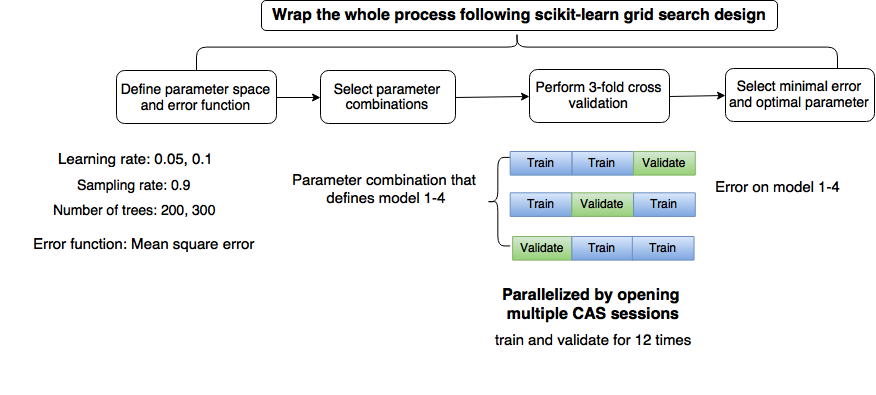
\includegraphics[width=12.5cm]{HyperparameterOptimization.png}
\end{figure}


%To solve this binary classification problem, we will follow the general machine learning pipeline. The first step is to generate new features from raw data(including stratifying and sampling). Then build machine model and do hyperparameter selection (grid search, bayes search, etc.). Last, ensemble several models based on train data and make a prediction of test data.

%We will focus on feature engineering, sampling and machine learning model. For feature engineering, we will do data exploration and feature reduction, the size of raw data is large(15.4GB) and doesn't fit into a single machine without feature reduction. The goal is to fit important features into a single memory with 16GB memory. For sampling, we will testify different methods such as upsampling, downsampling and SMOTE to process the highly imbalanced data(6879:1176868). For machine learning model, we will firstly use gradient boosting tree and then compare its performance with other machine learning models. We will testify three implementations of speeding up gradient boosting tree: Xgboost, FastBDT and SAS Viya. We want to get some insights how to improve the performance of gradient boosting tree for imbalanced data.

\section{Experiment}
In our experiment, the highest score we got in public board now is 0.19 for SAS Viya
\subsection{equal binning vs. quantile binning}

Single machine version of xgboost uses exact greedy algorithm that searches overall possible candidates, this can be desirable for deeper trees, and is usually what the user want. But this will slow the training speed when the number of observations is very large. So the gradient boosting implementation In the competition, we do data exploration in different numeric features. We find that some features are normally distributed and others are quite skewed, the distribution of some features are shown below. That's the reason xgboost outperforms SAS Viya, SAS Viya only supports equal binning. 
\begin{figure}[h]
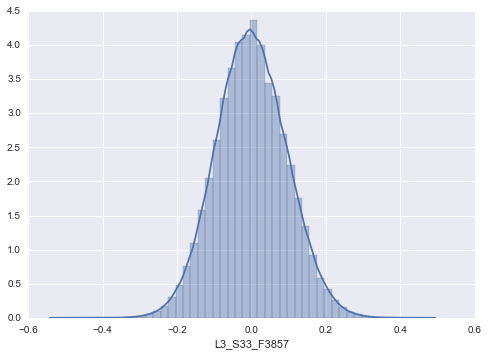
\includegraphics[width=10cm]{L3_S33_F3857.png}
\end{figure}

Skewed numeric feature
\begin{figure}[h]
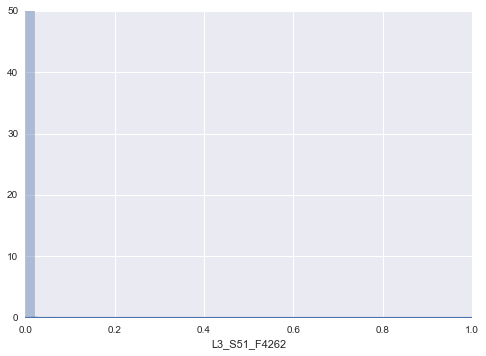
\includegraphics[width=10cm]{L3_S51_F4262.png}
\end{figure}

\subsection{Feature Importance}
We can get feature importance from numeric data.
\begin{figure}[h]
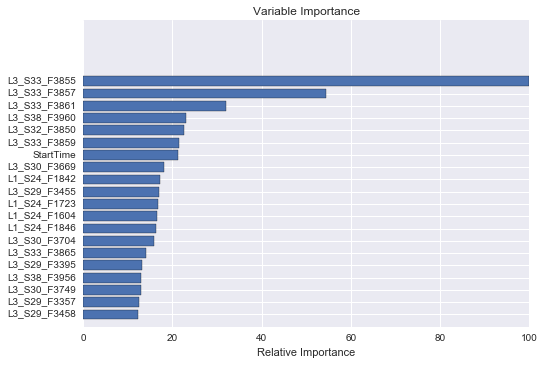
\includegraphics[width=10cm]{featureImportance.png}
\end{figure}

\section{Reference}

%[1] Chawla, Nitesh V., et al.(2002) SMOTE: synthetic minority over-sampling technique. {\it Journal of artificial intelligence research}, , pp.\ 321--357.

[1] Tianqi Chen,\ \& Carlos Guestrin. \ (2016) XGBoost: A Scalable Tree Boosting System. {\it KDD.}

[2] Keck T. \ (2016) A speed-optimized and cache-friendly implementation of stochastic gradient-boosted decision trees for multivariate classification {\it arXiv preprint arXiv}: 1609.06119.

[3] Chawla, Nitesh V., et al.(2002) SMOTE: synthetic minority over-sampling technique. {\it Journal of artificial intelligence research}, , pp.\ 321--357.



\section{Teammate and Work Division}

Xi \& Yeojin: Data exploration and feature reduction, sampling

Weijie \& Liang: Tree building, hyperparameter optimization

% Xi: Data exploration and feature reduction for categorical data, SMOTE

% Liang: SAS Viya machine learning pipeline, Tree building for imbalanced data

% Weijie: Employ and compare xgboost and FastBDT, hyperparameter optimization

% Yeojin: Data exploration and feature reduction for date data, upsampling and downsampling


\end{document}
